\section{Ergebnisse der Hyperparameter-Optimierung und des Trainings}
\subsection{Hyperparameter-Optimierung von \MiniDog{}}

In \autoref{fig:hyper-param} ist das Ergebnis der Hyperparameter-Optimierung von \MiniDog{}
dargestellt. Die optimalen Hyperparameter sind eine \texttt{Batch Size} von 2,
eine Stärke von 0.001 der \texttt{L2-Regularisierung} und die Verwendung
der Farbinformationen.

\begin{figure}
  \centering
  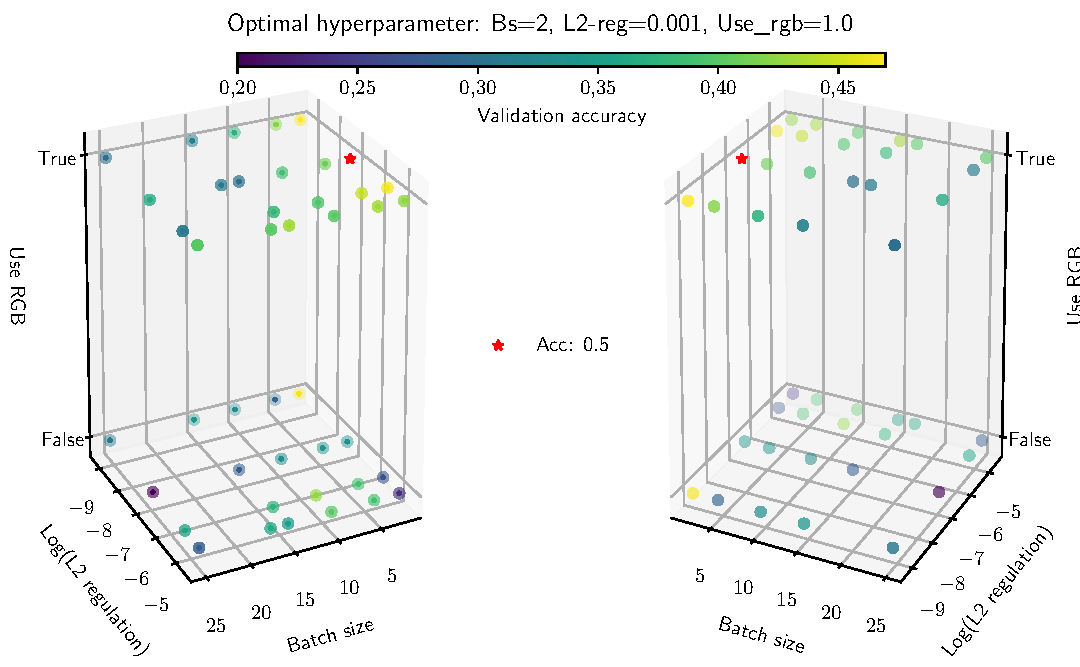
\includegraphics[scale=0.6]{pics/ergebnisse/hyper_raum.pdf}
  \caption{Darstellung der Ergebnisse der Hyperparameter-Optimierung
  von \MiniDog{}. Die beste Kombination ist als Stern dargestellt und wurde auch
  für das Training verwendet.}
  \label{fig:hyper-param}
\end{figure}

Allgemein wird ersichtlich, dass in den meisten Fällen die Verwendung von Farbinformationen
zu einer höheren Validation Accuracy führt. Folgerichtig optimiert die Verwendung
von Farbinformationen die Genauigkeit.

\subsection{\MiniDog}

% \begin{wrapfigure}{r}{11.2cm}
% \begin{figure}
%   \centering
%   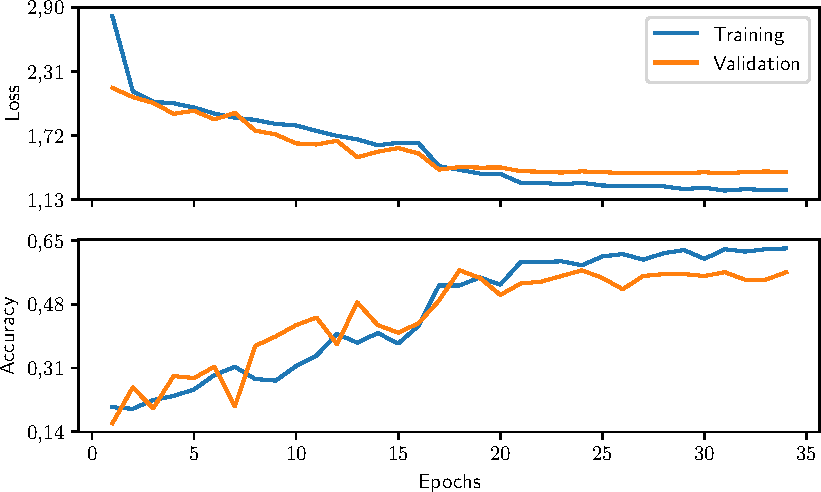
\includegraphics[scale=0.8]{pics/ergebnisse/MiniDogNN/history.pdf}
%   \caption{Loss und Accuracy Kurven für \MiniDog{}.}
%   \label{fig:loss-acc-minidog}
% \end{figure}
% \end{wrapfigure}

\begin{figure}
  \begin{subfigure}{0.49\textwidth}
    \centering
    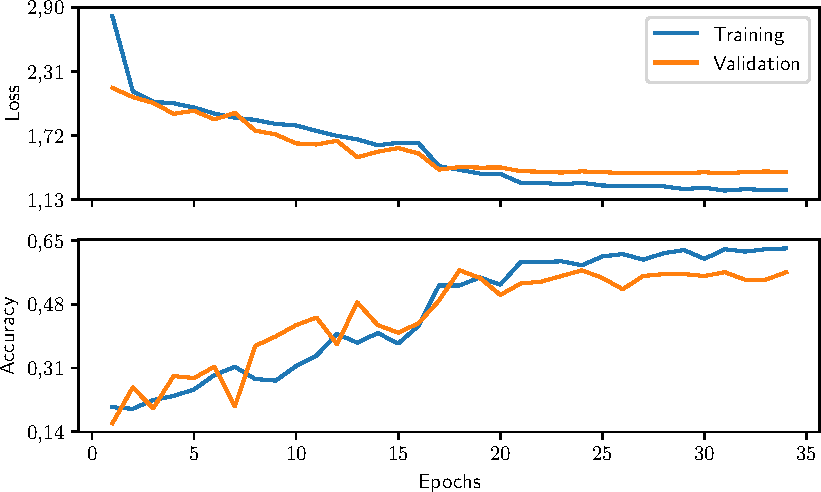
\includegraphics[width=\textwidth]{pics/ergebnisse/MiniDogNN/history.pdf}
    \caption{Loss und Accuracy Kurven für \MiniDog{}.}
    \label{fig:loss-acc-minidog}
  \end{subfigure}
  \qquad
  \begin{subfigure}{0.49\textwidth}
    \centering
    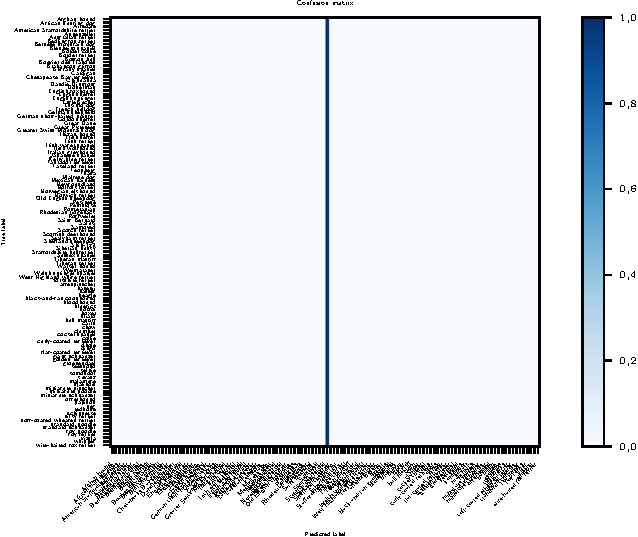
\includegraphics[width=\textwidth]{pics/ergebnisse/MiniDogNN/confusion_matrix_mini120.pdf}
    \caption{Confusion-Matrix für \MiniDog{}, trainiert auf 120 Klassen.}
    \label{fig:confusion-mini-120}
  \end{subfigure}
  \caption{Loss und Accuracy Kurven für den kleinen Datensatz und Confusion-Matrix
  für den großen Datensatz für \MiniDog{}.}
  \label{fig:mischmasch-minidog}
\end{figure}

In \autoref{fig:loss-acc-minidog} sind die Loss und Accuracy Kurven für \MiniDog{}
trainiert auf 5 Klassen zu sehen. Auch hier ist ab Periode 25 leichtes
Overtraining zu erkennen, welches mit stärkerer \texttt{L2-Regularisierung} oder
früherem Abbruch beseitigt werden könnte.

\autoref{fig:confusion-mini} zeigt die Confusion-Matrix des Trainings aus
\autoref{fig:loss-acc-minidog}. Es zeigt sich, dass der African Hunting Dog am
besten und der Chihuahua am schlechtesten klassifiziert wurde. Dies zeigt sich
auch in \autoref{fig:visualize-pred}. Dort wurde der Chihuahua am
wahrscheinlichsten als Beagle klassifiziert, was sich auch in der
Confusion-Matrix zeigt, da dort Chihuahuas mit gleicher Wahrscheinlichkeit als
Chihuahua oder als Beagle klassifiziert werden. Durch Optimierung z.\,B. der
Netzwerkarchitektur könnte man das Ergebnis noch verbessern, vor allem die Rassen
außer dem African Hunting Dog haben noch Verbesserungsbedarf.

In \autoref{fig:confusion-mini-120} ist die Confusion-Matrix von \MiniDog{} für
120 Klassen dargestellt ist. Es wird sofort ersichtlich, dass die Klassifikation
nicht gut funktioniert hat, da alle Bilder einer einzelnen Klasse zugeordnet
werden. Damit wird auch klar, dass nicht mit dem gleichen Netz 5 und 120 Klassen
gut klassifiziert werden können. Der Grund dafür liegt hauptsächlich darin, dass
der \CNN{}-Anteil von \MiniDog{} 64 Features generiert und trotz der Variation
des \FNC{} somit zu wenige Gewichte für eine 120-Klassen-Klassifikation vorliegen.

\begin{figure}
  \begin{subfigure}{0.49\textwidth}
    \centering
    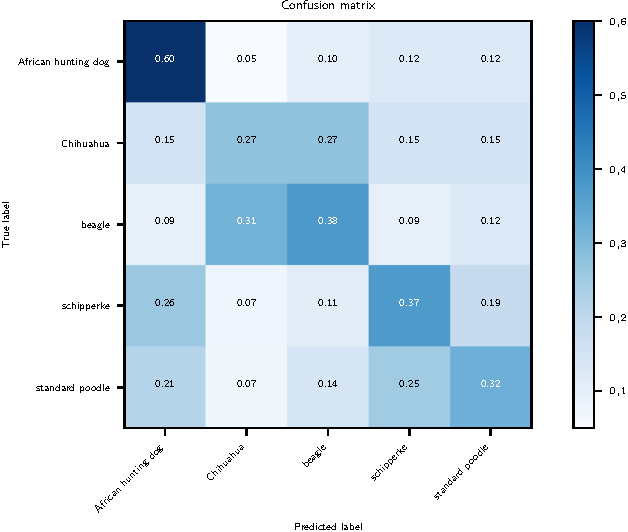
\includegraphics[width=\textwidth]{pics/ergebnisse/MiniDogNN/confusion_matrix}
    \caption{Confusion-Matrix für das Training von \MiniDog{}.}
    \label{fig:confusion-mini}
  \end{subfigure}
  \begin{subfigure}{0.49\textwidth}
    \centering
    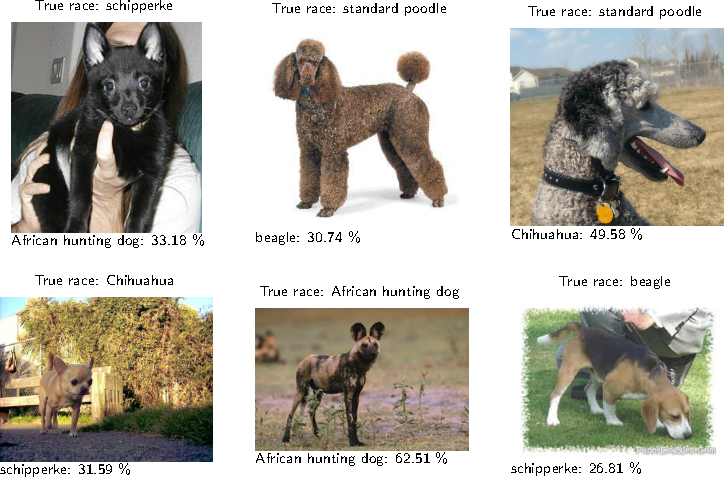
\includegraphics[width=\textwidth]{pics/ergebnisse/MiniDogNN/visualize_predictions.pdf}
    \caption{Auswahl von sechs Bilder aus dem Testdatensatz des kleinen
    Datensatzes für \MiniDog{} mit den jeweilig wahrscheinlichsten Predictions.}
    \label{fig:visualize-pred}
  \end{subfigure}
  \caption{Confusion-Matrizen für \MiniDog{} für den kleinen und den großen Datensatz.}
  \label{fig:confusion-mini-gesamt}
\end{figure}

% \begin{figure}
%   \centering
%   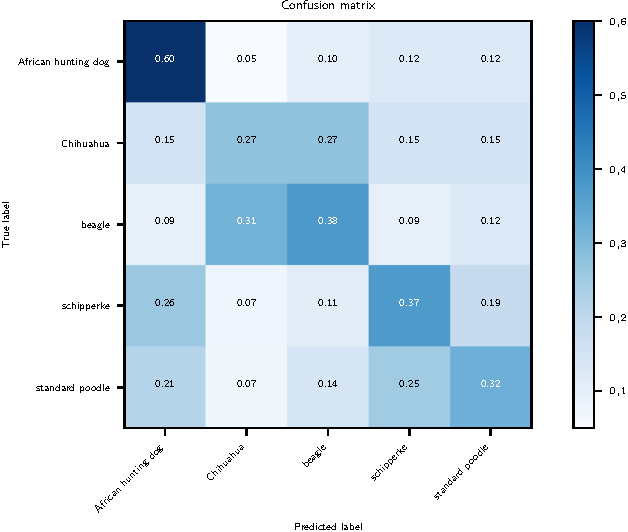
\includegraphics[scale=0.8]{pics/ergebnisse/MiniDogNN/confusion_matrix}
%   \caption{Confusion-Matrix für das Training von MiniDogNN.}
%   \label{fig:confusion-mini}
% \end{figure}

% \begin{figure}
%   \centering
%   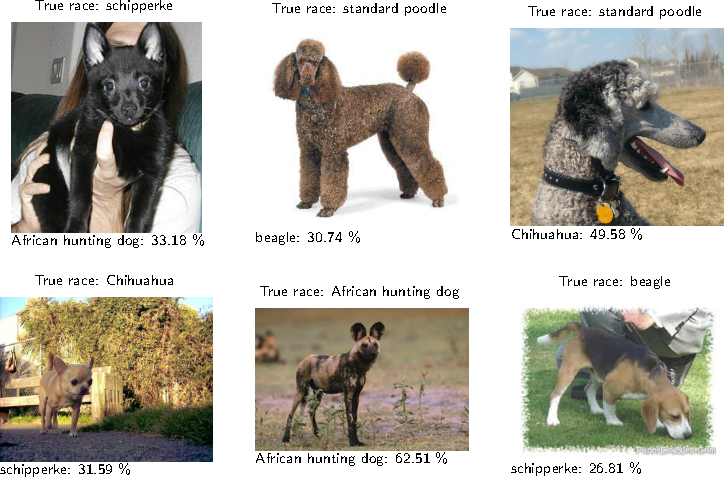
\includegraphics[scale=0.8]{pics/ergebnisse/MiniDogNN/visualize_predictions.pdf}
%   \caption{Auswahl von sechs Bilder aus dem Testdatensatz des kleinen
%   Datensatzes für \MiniDog{} mit den jeweilig wahrscheinlichsten Predictions.}
%   \label{fig:visualize-pred}
% \end{figure}

% \begin{figure}
%   \centering
%   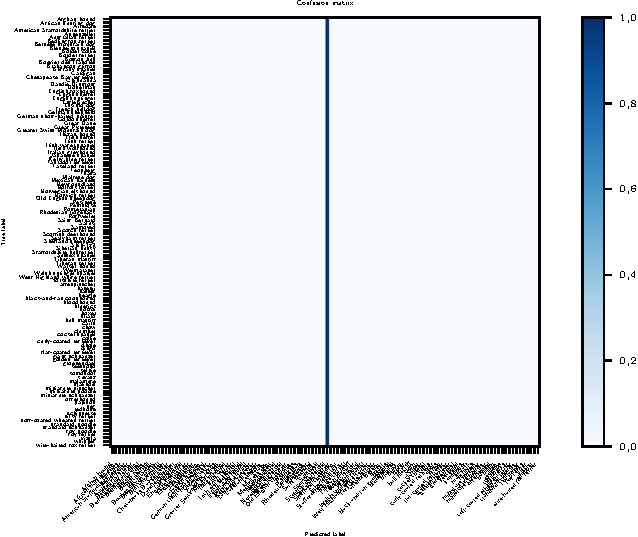
\includegraphics{pics/ergebnisse/MiniDogNN/confusion_matrix_mini120.pdf}
%   \caption{Confusion Matrix für \MiniDog, trainiert auf 120 Klassen.}
%   \label{fig:confusion-mini-120}
% \end{figure}

\subsection{Verschiedene Bildgrößen beim  Training von \PreDog{} und \PreBig{}}

Wie bereits in \autoref{sec:größe-bilder} beschrieben, wurde für die beiden
Architekturen, die ein vortrainiertes Netz nutzen, alle Bilder auf 224x224
reskaliert. Dies erreichte eine Validation Accuracy von ungefähr
\SI{95}{\percent}. Dadurch werden zwar 1735 Bilder des Datensatzes hochskaliert,
da aber beim Skalieren auf die minimalen Größen der beiden Datensätze die
Accuracy z.\,B. bei \PreDog{} auf ungefähr \SI{60}{\percent} (vgl.
\autoref{fig:loss-acc-kleine-groesse}) sinkt, wird 224x224 als Größe verwendet.
% Falls die Bilder aber auf 224x224 reskaliert werden, dann steigt die Accuracy
% auf ungefähr \SI{95}{\percent}. Da im kleinen Datensatz nur maximal 74 Bilder
% kleiner sind als 224x224, die Validation Accuracy aber deutlich besser ist, wird diese Methode zum Training verwendet.
% Loss und Accuracy Kurven sind im Anhang zu finden.

\subsection{\PreBig{}}

% \begin{wrapfigure}{r}{11.2cm}
%   \centering
%   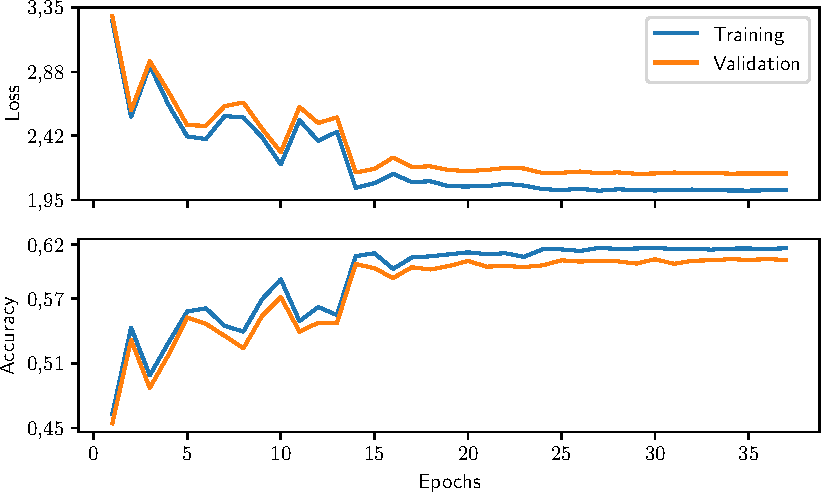
\includegraphics[scale=0.8]{pics/ergebnisse/PreBigDogNN/history_epoch.pdf}
%   \caption{Loss und Accuracy Kurven für \PreBig{}.}
%   \label{fig:loss-acc-prebig}
% \end{wrapfigure}

\begin{figure}
  \begin{subfigure}{0.49\textwidth}
    \centering
    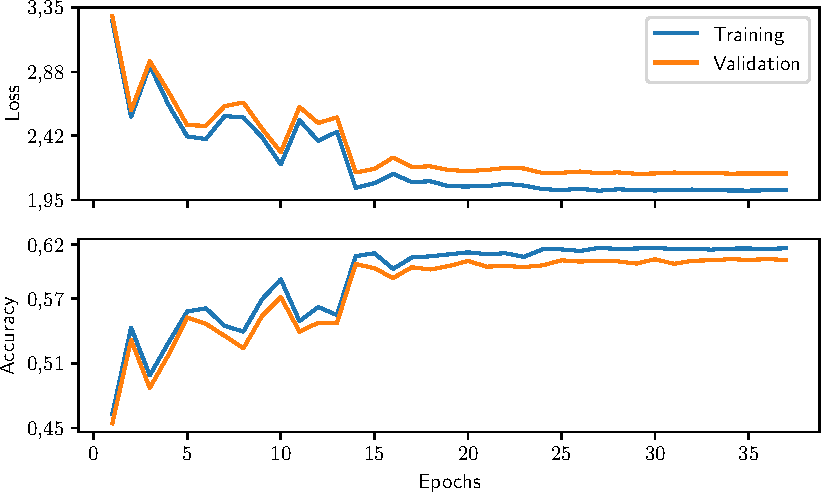
\includegraphics[width=\textwidth]{pics/ergebnisse/PreBigDogNN/history_epoch.pdf}
    \caption{Loss und Accuracy Kurven für \PreBig{}.}
    \label{fig:loss-acc-prebig}
  \end{subfigure}
  \qquad
  \begin{subfigure}{0.49\textwidth}
    \centering
    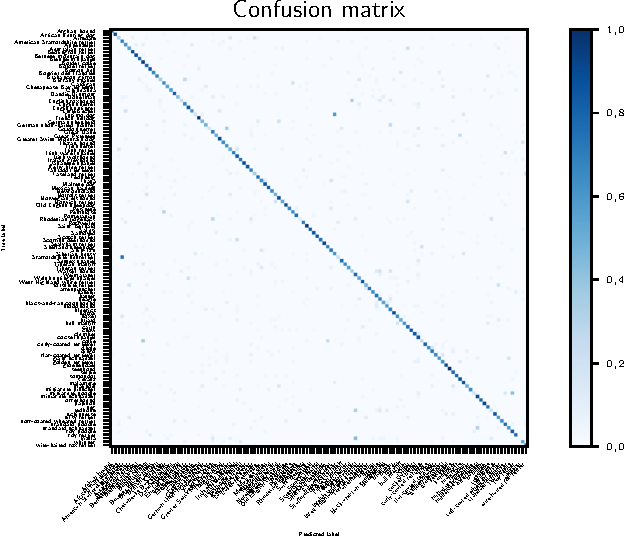
\includegraphics[width=\textwidth]{pics/ergebnisse/PreBigDogNN/confusion_matrix.pdf}
    \caption{Confusion-Matrix für \PreBig{}.}
    \label{fig:confusion-prebig}
  \end{subfigure}
  \caption{Loss und Accuracy Kurven und die Confusion-Matrix für \PreBig{}.}
  \label{fig:plots-prebig}
\end{figure}

In \autoref{fig:loss-acc-prebig} sind die Loss und Accuracy Kurven für \PreBig{}
zu sehen. Ungefähr ab Epoche 14 ist leichtes Overtraining zu erkennen. Hier
wäre eine Anpassung der \texttt{dropout-rate} und der Stärke der \texttt{L2-Regularisierung}
mögliche Stellschrauben, um das Overtraining zu beseitigen.

Die Confusion-Matrix zeigt eine deutliche Diagonale, was für eine hohe
Genauigkeit spricht. Allerdings werden einzelne Klassen häufig falsch
klassifiziert, zum Beispiel ist ein vom Netz als American Staffordshire Terrier
klassifizierter Hund zu ungefähr \SI{80}{\percent} ein Staffordshire
Bullterrier. Die Ähnlichkeit der beiden Rassen steckt schon im Namen und wird
bei genauerer Betrachtung der Bilder deutlich.

Zusammenfassend zeigt die Klassifikation eine hohe Genauigkeit,
einzelne Klassen wie z.\.B. der African Hunting Dog werden mit fast \SI{100}{\percent}-tiger
Wahrscheinlichkeit richtig klassifiziert.

% \begin{figure}
%   \centering
%   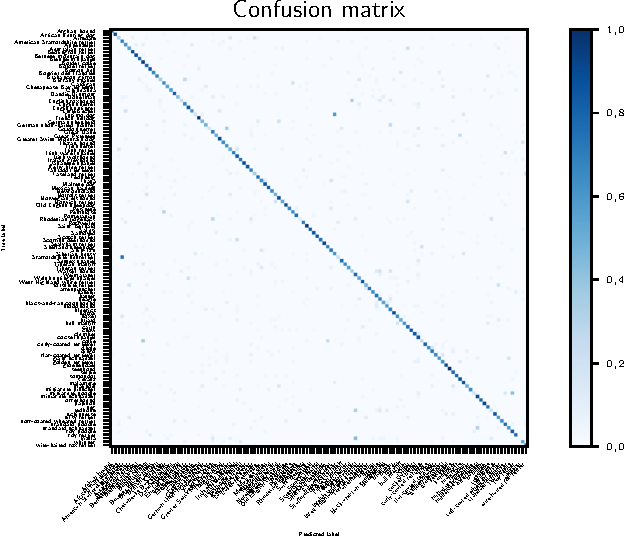
\includegraphics[scale=0.8]{pics/ergebnisse/PreBigDogNN/confusion_matrix.pdf}
%   \caption{Confusion-Matrix für \PreBig{}.}
%   \label{fig:confusion-prebig}
% \end{figure}


\subsection{\PreDog}

% \begin{figure}
%   \centering
%   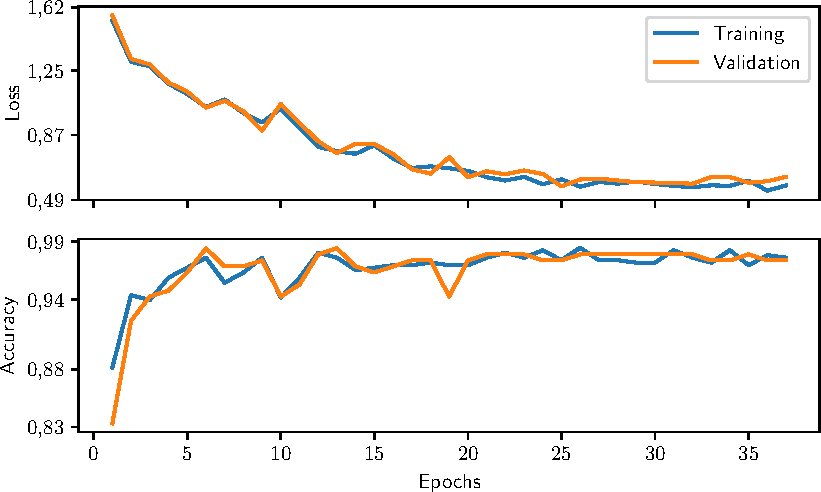
\includegraphics[scale=0.8]{pics/ergebnisse/PreDogNN/history_epoch.pdf}
%   \caption{Loss und Accuracy Kurven für \PreDog{}.}
%   \label{fig:loss-acc-predog}
% \end{figure}

\begin{figure}
  \begin{subfigure}{0.49\textwidth}
    \centering
    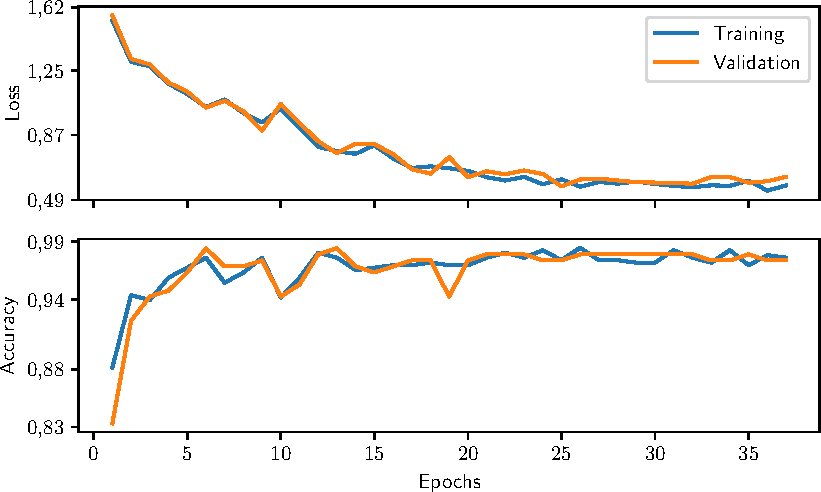
\includegraphics[width=\textwidth]{pics/ergebnisse/PreDogNN/history_epoch.pdf}
    \caption{Loss und Accuracy Kurven für \PreDog{}.}
    \label{fig:loss-acc-predog}
  \end{subfigure}
  \qquad
  \begin{subfigure}{0.49\textwidth}
    \centering
    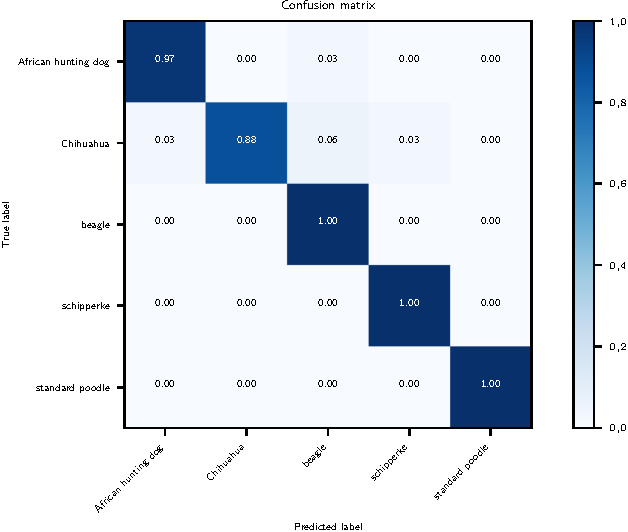
\includegraphics[width=\textwidth]{pics/ergebnisse/PreDogNN/confusion_matrix.pdf}
    \caption{Confusion-Matrix für \PreDog{}.}
    \label{fig:confusion-predog}
  \end{subfigure}
  \caption{Loss- und Accuracy Plots und die Confusion-Matrix für \PreDog{}.}
  \label{fig:plots-predog}
\end{figure}

In \autoref{fig:loss-acc-predog} sind die Loss und Accuracy Kurven für \PreDog{} zu sehen.
Es ist kein Overtraining zu erkennen, was als positiv zu bewerten ist.

Die Confusion-Matrix in \autoref{fig:confusion-predog} zeigt, dass das Training sehr gut
verlaufen ist. Beagle, Schipperke und Standard Poodle werden mit \SI{100}{\percent}-tiger
Wahrscheinlichkeit richtig erkannt; bei African Hunting Dog und Beagle werden teilweise
falsche Klassifizierungen vorgenommen, allerdings nur \SI{3}{\percent} bzw.
\SI{12}{\percent}. Somit lässt sich sagen, dass unter Verwendung des vortrainierten
Netzes die Klassifikation deutlich präziser verläuft als bei \MiniDog{}.

% \begin{figure}
%   \centering
%   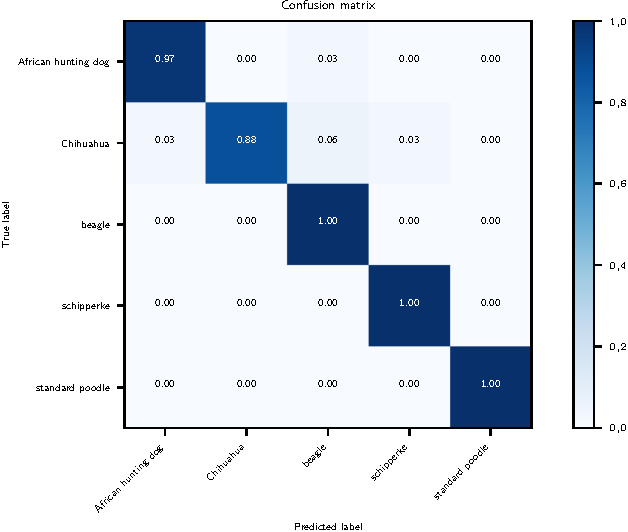
\includegraphics[scale=0.8]{pics/ergebnisse/PreDogNN/confusion_matrix.pdf}
%   \caption{Confusion-Matrix für \PreDog{}.}
%   \label{fig:confusion-predog}
% \end{figure}

\subsection{\texttt{Random Forest}}
In \autoref{fig:loss-acc-rf} sind die Loss und Accuracy Kurven für den
Autoencoder des Random Forest dargestellt.
% \begin{figure}
%   \centering
%   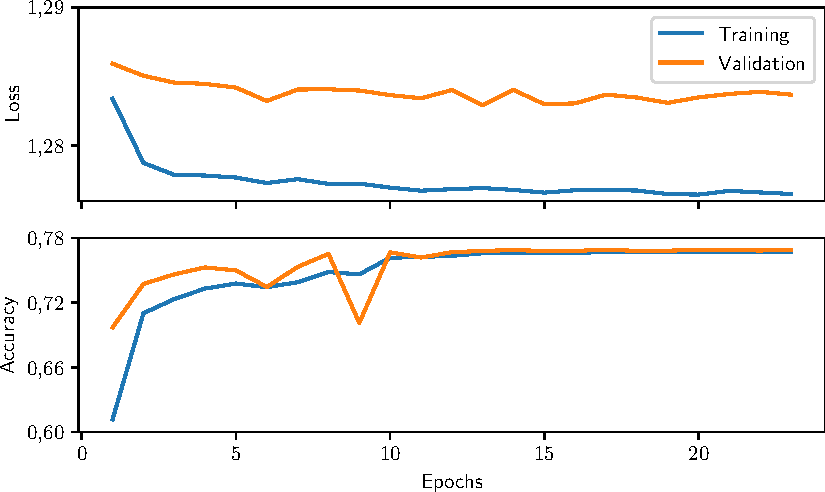
\includegraphics[scale=0.8]{pics/ergebnisse/RF/history.pdf}
%   \caption{Loss und Accuracy Kurven für den Autoencoder des Random Forest,
%   trainiert auf 120 Klassen.}
%   \label{fig:loss-acc-rf}
% \end{figure}
% \FloatBarrier
\begin{figure}
  \begin{subfigure}{0.49\textwidth}
    \centering
    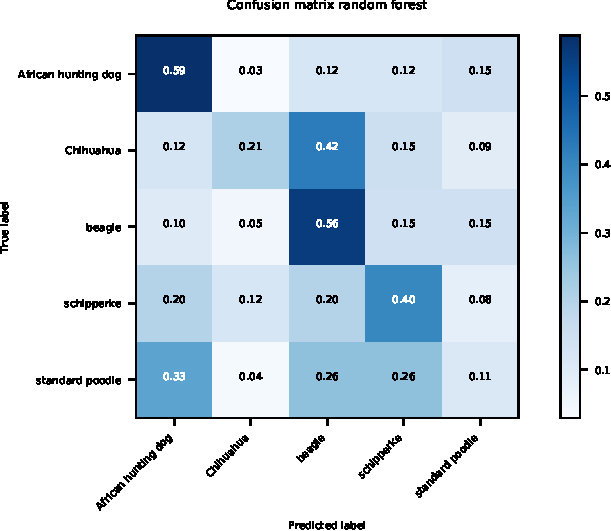
\includegraphics[width=0.92\textwidth]{pics/ergebnisse/RF/confusion_matrix_rf.pdf}
    \caption{Confusion-Matrix für die Klassifizierung des Random Forest auf 5 Klassen.}
    \label{sub:confusion-rf-5}
  \end{subfigure}
  \qquad
  \begin{subfigure}{0.49\textwidth}
    \centering
    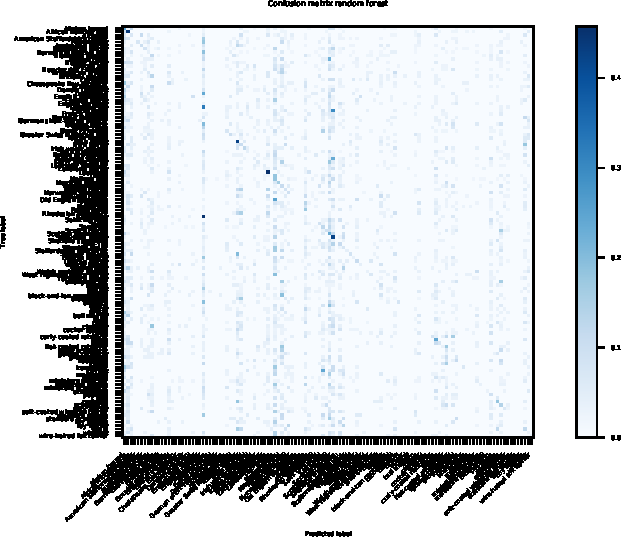
\includegraphics[width=0.92\textwidth]{pics/ergebnisse/RF/confusion_matrix_big.pdf}
    \caption{Confusion-Matrix für die Klassifizierung des Random Forest auf 120 Klassen.}
    \label{sub:confusion-rf-120}
  \end{subfigure}
  \caption{Darstellung der Confusion-Matrizen für 5 und 120 Klassen.}
  \label{fig:confusion-rf}
\end{figure}
% \FloatBarrier
Dabei wurde der Autoencoder auf dem
gesamten Datensatz trainiert. Aus der Loss-Kurve wird ersichtlich, dass
Overtraining vom Start weg gegeben ist. Es erscheint jedoch stärker als es ist,
da die Skalierung der y-Achse sehr fein gewählt ist. In der Accuracy ist dieses
Overtraining aufgrund der gröberen Skalierung nicht sichtbar; dies bestärkt die
Annahme, dass das Overtraining klein ist.
Die Confusion-Matrizen aus \autoref{fig:confusion-rf} zeigen, dass einerseits
die Klassifizierung für den großen Datensatz in \autoref{sub:confusion-rf-120} besser funktioniert hat
als bei \MiniDog{} (vgl. \autoref{fig:confusion-mini-120}), aber andererseits schlechter als bei
\PreBig{} (vgl. \autoref{fig:confusion-prebig}). Die Confusion-Matrizen für den kleinen Datensatz
sind schwieriger zu vergleichen im Hinblick auf \MiniDog{}, allerdings wird auch
hier ersichtlich, dass die Klassifikation mit einem vortrainierten Netz deutlich
besser funktioniert als bei \MiniDog{} (vgl. \autoref{fig:confusion-mini}) und
\autoref{sub:confusion-rf-5}.
